\subsection{Motivation}
    Imagine the following scenario: An overloaded system starts taking longer and longer to execute instances, for \texttt{worker\_1} it would take 10 seconds to complete an execution, OpenTelemetry \texttt{?end\_span} would only export the span after 10 seconds, thus, the system engineer would not know until 10 seconds after that htere is a problem in its system.
    \begin{center}
        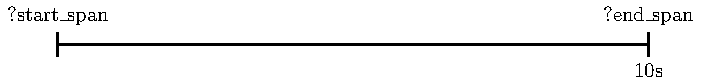
\includegraphics[width=\textwidth, scale = 0.8]{tikz/start_end.pdf}
    \end{center}
    This is problematic, why...

    Now, an engineer, knowledged about the system, knows that an execution of \texttt{worker\_1} should take maximum 1 second, after that, an execution ... [i dont know]
    \begin{center}
        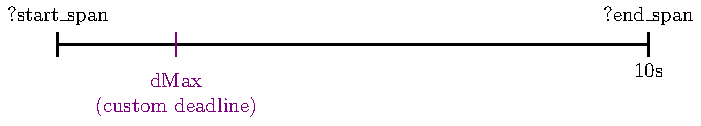
\includegraphics[width=\textwidth, scale = 0.8]{tikz/start_end_dmax.pdf}
    \end{center}
    In this case, the engineer who is using the oscilloscope would instantly get notified of the execution deviating from normality.


